\documentclass{cce2014-design}
\svnInfo $Id: design_brief.tex 7877 2024-03-12 16:30:22Z jrou0001 $

% Packages
\usepackage{tikz}

\usepackage{url}
\usepackage{amsmath}

% Document details
\title{Design Brief: Group 4}
\author{Keith Farrugia, Gabriel Vella, Alessandro Parrella, Jonas
   Rousseau-Morvan }
\date{\svnMaxToday, Document v.\svnInfoMaxRevision}
\begin{document}

\maketitle

\abstract{
	The project is on the creation of a DTMF (Dual tone multi-frequency) decoder
	using the ARM Cortex-M4 microcontroller.
}


% ==============================================================================
%                                  Introduction                                 
% ============================================================================== 
\section{Introduction}
The project's goal is the implementation of a DTMF decoder. It requires the 
implementation of an analog audio input and an LCD screen output. The general 
concept is that a line level output from a device is converted to a readable
analog signal which is in turn sent through an analog-to-digital converter (ADC)
to be transformed into a constant byte stream. The system will then use buffers
to store the output of the ADC which are set at suitable sizes to ensure 
accurate values, the minimum value being enough to capture a single period of 
the lowest frequency wave. 

The buffer is then fed to a  Goertzel algorithm that will decompose the signal 
into the frequencies making up the DTMF range. Through the use of a threshold
the system is able to decipher which DTMF signals are being sent, if any, 
taking only at most 2 signals at a time else the sample is deemed invalid. 
The signals are then mapped to the keypad where the LCD is used to display 
the output (e.g.\ if we have a 697Hz and a 1209Hz signal the LCD will be 
displaying 1). The whole application will be multithreaded so that we can 
read the input, decode and display the required information as well as
any input polling, at the same time. The implementation will be coded and 
implemented with use of Keil MDK and the provided drivers such as GPIO.


% ==============================================================================
%                                 System Design                                 
% ============================================================================== 
\section{System Design}

\subsection{Conceptual Overview}
This section will contain most of the theory-related concepts. It consists of
a general overview of how parts were being tackled making use of diagrams and
occasionally pseudocode.

\subsubsection{ADC Buffer Size}
In our original idea we planned on using buffers of 32 samples to contain at
least one period of signal. We based our reasoning on equation~\ref{eq:1}.
\begin{equation} \label{eq:1}
	B = \frac{x}{f_l}\cdot\frac{1}{s}
\end{equation}
This equation has $B$ the buffer size (in terms of number of samples — irrelevant
of the actual size of those samples, one byte, 16-bits, 32-bits — or any other),
$x$ is the \textit{Analog-to-Digital-Converter} (ADC) sample rate which is
expressed in bits per second ($b\cdot{}s^{-1}$), $f_l$ is the lowest frequency
we want to capture (since the lowest frequency means the highest period). This
equation should have supposedly given us the minimal acceptable buffer size for
capturing the kind of signal we want. This can be proven using dimensional
anlysis\cite{MIT-DA}, as shown in equation~\ref{eq:2}. Here the brackets
represents the \textit{dimension} — in the physical meaning of the word — of the
variables.
\begin{align}
	\begin{split}\label{eq:2}
		[B] &= \frac{[x]}{[f_l]}\cdot\frac{1}{[s]}\\
		samples &= \frac{bits\cdot{}s^{-1}}{Hz}
		\cdot\frac{1}{bits\cdot{}samples^{-1}}\\
		samples &= bits \cdot \frac{samples}{bits} \\
		samples &= samples
	\end{split}
\end{align}
The lowest frequency of the DTMF specification being 697Hz, we had run the
computation and obtained that we needed \textit{at least} 20 sample, which we
rounded to 32 to ensure precision and to have a sample size which was a power of
two. However, in practise after running several tests in a Jupyter Notebook we
used to simulate the attended behavior of our DTMF-microcontroller program (this
was useful as it permitted to run test before implementing a somewhat heavy
program on the microcontroller and try to understand what happened afterwards)
we discovered that even though 32 samples worked, we had a poor precision usig
this size for our samples buffer. For this reason, we chose to use a buffer size
of 256 samples to increase the precision of the results.

\subsubsection{ADC Sampling}
The current adc.c file in drivers provides the facility to read a singular
analog value from the ADC pin (pin 23)\cite{LPC4088} \cite{BaseBoard}. 
In the previous section (ADC sampling) the sampling rate and buffer size 
for adequate sampling were mentioned.

The sampling for the data needs to happen in a parallel fashion to the other
programs running on the microcontroller. This is because samples need to be
taken at consistent intervals. This calls for some sort of multi-threading to be
implemented which will be discussed in the next section. Therefore, 2 buffers are
needed; one to be filled by input and another to be decoded. These will be
switched by the two threads once both are finished with their current buffer.

In terms of physical signal processing, the audio output will not be directly
connected from the relative output device to the controller's ADC pin. A circuit
such as the one implemented in [Figure 1] in the handbook will likely be used to
shift the voltage to be in the range of "VREF" (3.3V) and 0V.

On a similare note the sample rate choosen for the system is that of 8000 Hz.
Theoretically by according to the Nyquist theorem for an accurate sample it is
best to sample at twice the highest expected frequency. Given that the highest
frequency in the system is that of 1633 Hz then the double would be 3266Hz.
Although this would have technically been a suitable frequency it was decided
to follow the more practical and standard sampling rate of 8000Hz \cite{itu-g711}.

\begin{figure*}[t]
	\center
	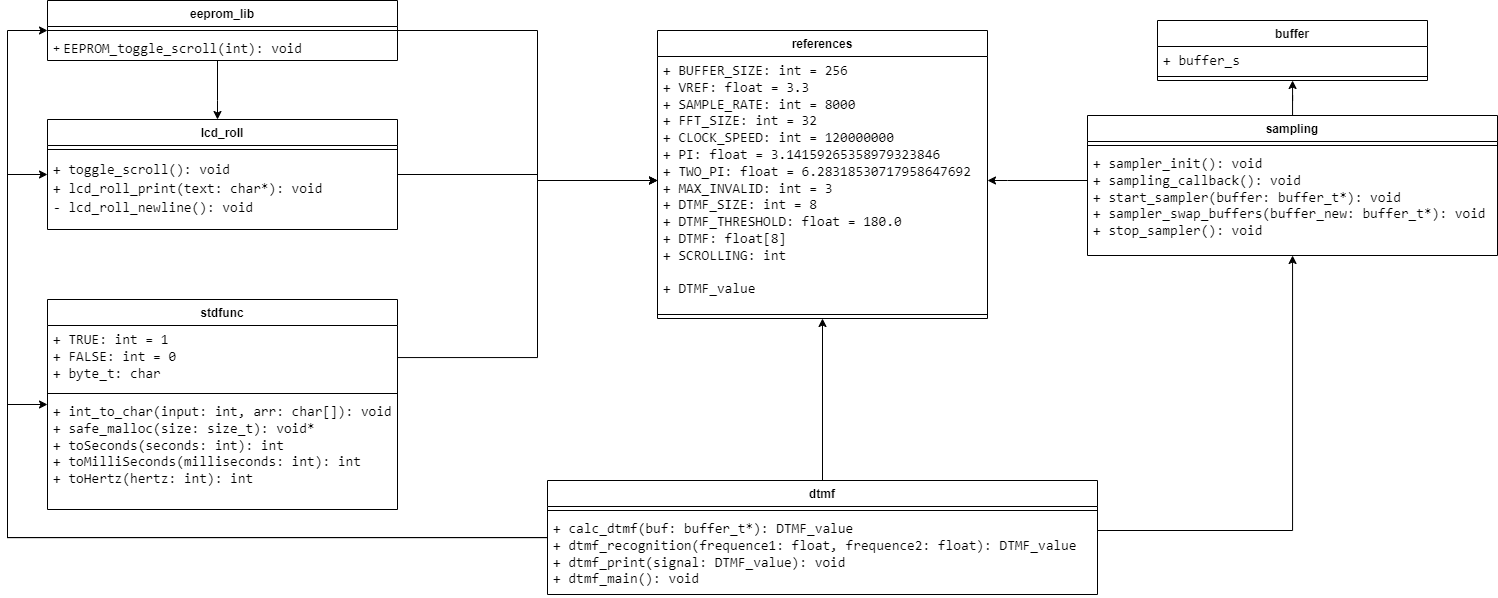
\includegraphics[width=\textwidth]{img/UML DTMF.png}
    \caption{\label{UMLdiag}UML Class Diagram}
\end{figure*}

\subsubsection{Threading \& Interrupts}
In order for the system to function reliably a multithreaded implementation 
is needed. However, the execution does not need to be as robust or as complex
as something along the lines of an operating system. The current system is
based on interrupts, more specifically the callback functionality provided by
the timer driver. By setting the timer to call a specific function when a time
equivalent to the sampling frequency passes, it is possible to interrupt the
main thread and allow for consistent sampling to take place.

There are other systems that could have benefitted from interrupt handling, mostly
ones related to I/O such as button presses. However, it was deemed that a simple
polling implementation for such events would be sufficient due to their low priority
and due to them not being intensive tasks.

\subsubsection{Goertzel Algorithm}
Once the audio signals are sampled and digitized through the ADC, the digital
samples must be analyzed to identify the frequency components, either using the
DFT \cite{goertzel} or the FFT \cite{fft}. Both of these functions serve
the same purpose, with the primary difference being their computational
efficiency (i.e. cpu intensive) and the simplicity of implementation (the FFT 
being more complex). The decision needs to be based on the system's resources,
implantation complexity and the specific requirements of the DTMF detection.

It was for these reasons the Goertzel was chosen as its implementation 
resulted in a lesser cpu cycle consumption as well as being a lot easier to
implement and debug. This also removed the need for post-processing of the 
generated signal range such as with interpolation as would have been needed
with FFT. This is because Goertzel works by giving magnitudes which denote
how present a specified frequency may be in a given sample. Therefore, the
algorithm will only compute for a specific set of given frequencies and nothing
else.

Another issue which was theoretically possible was that of distinguishing these
tones accurately in the presence of background noise or other distortions. In 
practice the low sample frequency in combination with how Goertzel functions
meant that noisy frequencies where almost altogether ignored given that noise
usually plays as an outlier on the higher end of the frequency range.

\subsubsection{LCD}
The board has a special connector named J11, designed to connect with a type of
display known as a character LCD. These displays are common and affordable,
showing text using a grid of characters (like letters and numbers). These
character LCDs connect and communicate with other devices (like the board)
using a set of wires that form a "bus." This bus can work in two ways: using 4
bits or 8 bits at a time to transfer data. Bits are the smallest units of data
in computing, so this is about how much information the display and the board
can send or receive at once. The board is set up to work in the 4-bit mode. This
means it sends and receives data in chunks of 4 bits. But, instead of connecting
directly with a bunch of wires (which would typically require more connections
for control signals), the board cleverly uses a shift register connected to
something called an SPI bus. An SPI bus is a common way for electronic devices
to talk to each other using a serial connection. It's like a streamlined
conversation where data is sent one bit after another, in a line, instead of all
at once (parallel). Thanks to the shift register (a type of circuit that can
take in data serially and then output it in parallel, or vice versa), the board
can communicate with the LCD using just three wires, even though the LCD is
designed to receive data in parallel. This setup simplifies the wiring and makes
it easier to control the LCD, saving space and resources on the board. The
following details can be observed:

\begin{itemize}
	\item SPI MOSI (P1.24): This pin is used for the SPI Master Out Slave In
        function. It is typically used to send data from the microcontroller to
	      the LCD.
	\item SPI SCK (P1.20): This pin represents the SPI Clock. It is used to
	    synchronize data transmission between the microcontroller and the LCD.
    \item LCD-RST (P0.23): This is the reset pin for the LCD. It is used to
        reset the LCD, which can be necessary when initializing the display or
        recovering from an error state.
	\item LCD-A0 (P0.25): This pin is labeled A0, which might be used as the
	    Register Select (RS) pin for the LCD (although this is not standard
	    naming). It is used to switch between sending commands or data to the
        LCD.
	\item SPI\_SSEL (SPI Slave Select) (P1.2): This pin is used to enable or
	    disable a specific device on the SPI bus.
	\item BL\_CTRL (Backlight Control) (P2.1): This pin controls the backlight
        of the LCD.
\end{itemize}


\subsection{Additional I/O Hardware}
The following hardware components where used: 
\begin{itemize}
    \item Capacitor (100n)
    \item Resistor (100)
    \item Resistors (100k) 
    \item 2 Diodes (1N4148)
\end{itemize}

A prototyping board will also be used to solder the line level input to
analogue converter circuit. This was to ensure that the circuit does not
break during transportation and more tightly secured.

\subsection{UML Diagram}
The UML Diagram in [Figure \ref{UMLdiag}] shows the structure of how the
components interact and make use of each other. The UML only lists the main
components and does not include external code such as drivers, code taken
the provided labs or code which is sourced externally

%============================== REQUIREMENT TABLES ============================

\subsection{System Requirments}

\subsubsection{Functional Requirments}
\begin{tabular}{|p{0.1\linewidth} | p{0.8\linewidth}|}\hline
	(F.1) & The system reads inputs and immediately decode and display the
	calculated values once a buffer is filled. Although this may be a slightly
    slow Computer, the delay is not noticeable to the user.
    \\ \hline
	(F.2) & The pull down button is used to switch between auto scrolling and non
    auto scrolling.
    \\ \hline
	(F.3) & The LED in the base board is used to display when the auto scroll has
    changed (blue), and notify the user when the error case is reached (red).
    \\ \hline
	(F.4) & The System makes use of Hitachi HD\_{44780}-based 2-line text
    LCD. 
    \\	\hline
	(F.5) & The program will start by initializing the different drivers followed by
    reading the EEPROM for the last user setting before finally starting the dtmf
    decoding.
    \\ \hline
	(F.6) & The system will store inside the EEPROM the last user setting related
    to scrolling.
    \\ \hline
	(F.7) & The LED will turn red upon reaching the error case which is when the sampler
    finds a full buffer because it was faster than the decoder.
    \\ \hline
	(F.8) & At no point do any error cases or invalid readings trigger an unstable state
    such as stopping the program.
    \\ \hline
\end{tabular}

\subsubsection{Technical Requirments}
\begin{tabular}{|p{0.1\linewidth} | p{0.8\linewidth}|}\hline
	(T.1) & The solution is based on the LPC4088 experiment bundle (as can be seen
	from the video).
    \\ \hline
	(T.2) & The solution is written entirely in C/C++.
    \\ \hline
	(T.3) & The solution is based on the uVision V5.39.0.0
    \\ \hline
	(T.4) & No third party libraries where used, except the provded
	drivers and the EEPROM third party driver code fragment from \cite{nxp-cdl}.
    \\ \hline
	(T.5) & The system uses its resources in a considerate manner with minimal wastage.
    \\ \hline
	(T.6) & The system is multithreaded with the use of the timer driver.
    \\ \hline
	(T.7) & The timer driver is what is used as an interrupt handler since the timer 
	itself causes an interrupt at which the interrupt handler (sampler) is called.
    \\ \hline
\end{tabular}

% ==============================================================================
%       Implementation
% ==============================================================================


\section{Implementation}
\subsection{Code Organisation}


\subsubsection{Coding convention}
To improve code quality and readability and to ensure that each one of us could
work with other's code, we decided to follow formatting rules such as naming
typedefing struct and redefined types with the \texttt{\_t} suffix, per example
the bool type (which is a redefinition of \texttt{int} but has been renamed to
create more meaningful codes) is defined as:
\begin{verbatim}
typedef int bool_t;
\end{verbatim}
A more complex type used to wrap frequency and magnitude for the goertzel
algorithm is defined this way:
\begin{verbatim}
	typedef struct
	{
	    float frequency;
	    float magnitude;
	} frequency_magnitude_t;
\end{verbatim}
Here we can see another one of our convention: ``reducing'' identifier as
little as possible, the \texttt{frequency} field could have been named
\texttt{freq}, but we chose to not reduce the identifier to ensure better
readability and avoid having pieces of code looking ``abstract'' as much as
possible. Those are just example of the convention we used, in the whole we
tried to stick to classic conventions (having constants/enum values in capitals,
using \texttt{\#define} calls in the header file, etc.) This permitted our code
to be universally readable to anyone with knowledge of the C language without
having to decipher badly formatted code. Of course, there may be some
irregularities (per example, function names are often snake-cased, sometimes
camel-cased) but, in the whole, we tried to stick as much as possible to our
conventions.

\subsubsection{File organisation}

The project file organisation was made following our module-based approach. The
file structure of the \texttt{trunk} directory was taken from the labs' file
structure with directories for the drivers, object files, a \texttt{.uvprojx}
file etc. We took directly those from one of the labs and only modified the
content of the \texttt{src} directory. This section will only focus on how we
organised our code inside that directory.

The \texttt{src} directory contains the source files of the project most of them
were written by us but not \textit{all} of them, per example, the subdirectory
\texttt{io} contains the files \texttt{lcd.h} and \texttt{lcd.c} which we took
directly from one of the labs to avoid reinventing the wheel. The different
subdirectories of \texttt{src} are :
\begin{itemize}
    \item \texttt{dtmf} which contains files whose content is related to
        recognizing and treating DTMF received signals ;
	\item \texttt{fourier} which contains the code of the Goertzel algorithm,
        it is named that way because we first wanted to implement the FFT
        algorithm ;
	\item \texttt{io} which contains all file whose content is used to handle
        input and output functions such as controlling the LCD, using switches,
        LEDs etc. ;
	\item \texttt{libraries} this directory is a catch-all directory, it was
        named this way because its initial use was to contain the
        \texttt{stdfunc.c} and \texttt{stdfunc.h} files which act as a
        ``standard'' library for our program ;
	\item \texttt{sampling} which contains files related to sampling and
        buffering the audio input.
\end{itemize}
The \texttt{src} directory also contains the \texttt{main.c} file which is the
program's entry point. Organizing our code this way allowed us to have a file
tree structure representing the way we thought about our program. Among the
different files of the \texttt{src} directory we believe that it is important to
dwell a bit on \texttt{references.h}, \texttt{stdfunc.h} and \texttt{stdfunc.c}
which can be found in the \texttt{libraries} subdirectory.

The \texttt{references.h} file contains global definitions, variables, structs
definitions, enums definitions etc.\ that must be available to the rest of the
files, for example, the buffer size can be needed in different modules, to avoid
re-defining globals in each module and reinforce code quality we chose to define
it in the \texttt{references.h} file. 

The \texttt{stdfunc.c} and \texttt{stdfunc.h} files contains generic functions
that found themselves useful during the programming process and that we thought
might be useful outside the module they were first needed in. Those include
generic mathematical function or strings-related functions like
\texttt{int\_to\_char()}. This does not mean that those functions are used in
multiple modules but that they were too generic to be put inside a specific
module.

For the content of the different modules (DTMF-recognition, Sampling, Goertzel
algorithm implementation, etc.) those will be discussed more deeply in other
sections of this report, so we believe there is no need to discuss them here. 

\subsection{DoxyGen}
It is important to note that the code repository is also able to generate a 
Doxygen report. The doxygen file can be found in code/trunk.src where the command 
"doxygen doxyfile" can be run in order to generate the doxygen report. 

Most files and functions contain doxygen comments including the drivers with some
excptions being the leds.h/leds.c and switches.h/switches.c. These where left as is
since they were optained from the labs provided.

\subsection{Sampling}
\begin{figure*}
	\center
	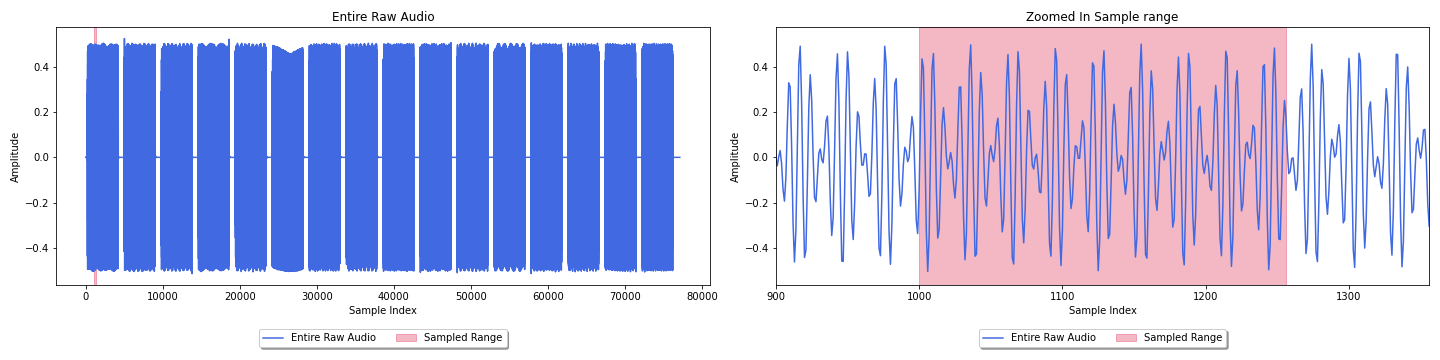
\includegraphics[width=\textwidth]{img/Sample Area.png}
	\caption{\label{SampleArea}Sample Area}
\end{figure*}
\begin{figure*}
	\center
	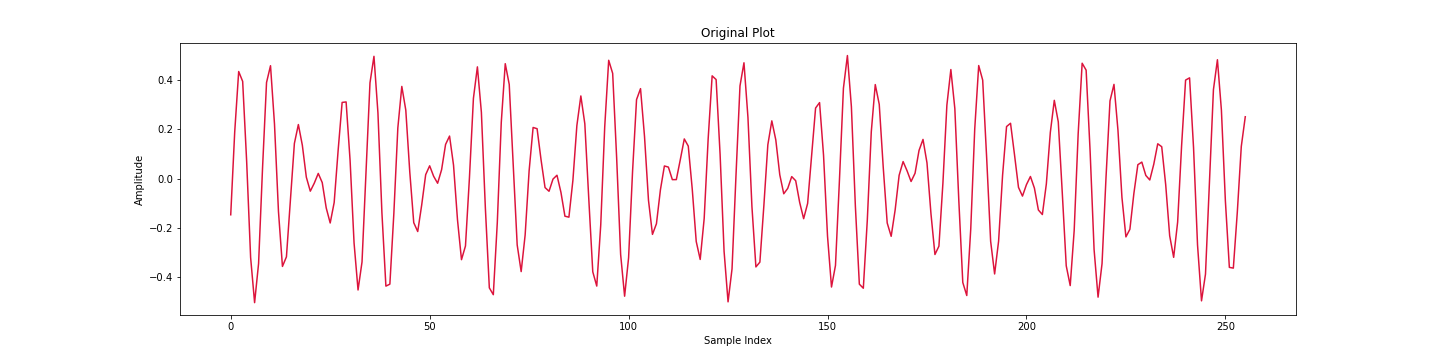
\includegraphics[width=\textwidth]{img/Sample.png}
	\caption{\label{Sample}Sample}
\end{figure*}
As mentioned in the Design Specification section, the sampling is done through
interrupts more specifically through the timer driver provided. Through
simulations in Python as well as through research, it was deduced that an 
effective sample rate was that of 8000Hz, with the number of samples being around 
256. The figure [Figure \ref{SampleArea}] shows an example of what extent of the 
original wave we are sampling. In the figure [Figure \ref{Sample}] the example 
sample that would have been taken from the sampled area is also shown. From this, 
it can be seen how the lower sample rate creates a more jagged wave but is still 
comparable to the original.

The Sampler makes use of the buffer\_t struct, which holds a sample buffer and
a boolean value. This struct is what is swapped between the decoding algorithm 
and the sampler each iteration. The sampler fills an element with struct's sample 
buffer with each timer callback until the buffer is full. It is at this point that 
it turns on the struct's boolean value which serves to notify the decoder that the 
sampler is done.

The reason why the sampler does not switch the buffers itself is to avoid the 
possibility that the buffers are switched during decoding. How it is currently set
up is that all control over the buffers is given to the main dtmf loop. If in the
case that the sampler has not finished sampling then the loop will simply wait until
it is finished. On the other hand if the suppler fills the buffer and the buffer has
not switch before its next sample, the sampler will launch an error case, triggering
the LED to turn red, and skipping the reading of that sample. The sampler will continue
skip readings until the buffers are swapped. Although this may seem crude it does give
the system more robustness as there is no chance that a buffer is overwritten while 
its being used.

\section{Decoding the Signal}
\subsection{Goertzel}
As stated before, during the practical implementation, it was decided that the 
frequency decoding/calculation should be done through the Goertzel algorithm 
\cite{goertzel}. This provided several benefits over the 
Fast Fourier or Cooley-Tukey implementations that were discussed during the 
planning of the project. Firstly the Goertzel Algorithm is overall simpler to 
implement, which would result in fewer bugs and errors that would reduce the 
need for a lot of decoding.

The source for the Goertzel can be found in the fourier folder. Although the
implementation may be slightly different from what the typical implementation,
it still performs the same calculation although some corners where cut for
performance.

It does also use an index instead of taking a given frequency, this is so that
the frequency can be taken from the gloabl array DTMF at wherever the index may
point to. There were attempts to also optimize the Goerztel so that the
coefficients would be calculated once on run time in a global array, but there 
were many issues with the array not keeping the updated state, so this was scraped
for the current implementation as this was sufficiently fast.

\subsection{DTMF}
calc\_dtmf is the next function in the chain. It is here that parseGoertzel 
is then called. The purpose of this function is to remove the frequencies 
that fall below the designated threshold and try to map a DTMF value to the 
2 highest frequencies. The mapping of the frequencies to a dtmf value is only 
done if exactly 2 frequencies reach the treshold. If no frequencies are above 
the treshold then the reading is designated as a quiet space which means that 
no key on the DTMF keypad was pressed. Else the sample is set as an invalid, this 
is so that if multiple DTMF signals are sent over the line then the reading would
be invalid. Once there are 2 valid frequencies then they are passed to a 
recognition function that maps them to the equivalent value in the DTMF keypad.
On a seperate note the magnitude treshold value waas decided through trial and
error after multiple runs with different input


The DTMF\_main function is where the main loop is repeated. The concept here 
is that the switching of buffers, controlling of output and decoding are all
controlled from this while loop. To swap the buffers the function creates an 
array of buffer\_t type of length 2 where using the modulus operator we can 
keep iterating between the first and second position of the array hence 
effectively switching the buffers.

The loop starts by first polling the switch input to check if the user wants to
stop or start scrolling. Its second job is to then wait for the sampler to finish 
reading where it then swaps the buffers to allow the sampler to continue. The 
function calls the calc\_dtmf function to calcualte and map the dtmf value. 
There are four cases which then follow;
\begin{itemize}
    \item If the dtmf value is equal to QUIET then this means that quiet a 
        region has been found at which point the counter is incremented. This is
        because a quiet space is not immediatly recogized but needs to appear
        for a certain amount of samples denoted by MAX\_QUIET.
    \item If the dtmf is read and is not the same as the previous dtmf value
        then this is printed to the LCD.
    \item If the dtmf is a repeating value then it is only dispalyed if a 
        recognized quiet space is recognized meaning that the user has let go
        and re-pressed the button.
    \item The final case is if the reading is invalid or just plain repetitive
        here the counter for the quiet region is simply reset.
\end{itemize}

\subsection{Switches}
The integrated joystick was used on the board to provide user input for 
toggling the autoscroll function on the LCD. Specifically, when the 
joystick is pulled downward, it polls the function that toggles the autoscroll 
mode on or off. This functionality allows users to control the display of decoded 
DTMF signals more efficiently, enabling them to view previous outputs without 
continuous scrolling. The polling mechanism ensures consistent monitoring of 
the joystick's state, allowing for timely response to user input. Additionally,
the state of the autoscroll mode is stored in the EEPROM to retain the setting 
even after a system reset or power cycle.

\subsection{LEDs}
The system uses an LED indicator to provide visual feedback to the user 
regarding the current state of the autoscroll function and buffer status. The LED 
is also toggled red every time the buffer is full and remains red until the 
buffers are swapped again. Each time the autoscroll mode is toggled using the 
joystick, the LED flashes blue to confirm the action. This immediate visual 
feedback helps the user understand that the mode has been successfully changed. 
The LED control is integrated with the polling mechanism for the joystick, 
ensuring that the LED flashes precisely at the moment of toggling. This feature 
enhances user interaction by providing clear and immediate visual cues 
about the system's operations and settings, ensuring that the user is always 
aware of the current state of the display settings.

\subsection{EEPROM}
The EEPROM functionality is implemented to store the autoscroll setting persistently. 
We adapted an EEPROM library found online \cite{nxp-cdl} to fit our specific 
requirements. This library was modified to integrate seamlessly with our system, 
allowing the autoscroll mode's state to be saved and retrieved from the EEPROM. 
Each time the joystick toggles the autoscroll function, the new state is written 
to the EEPROM. Upon system startup, the state is read from the EEPROM to restore 
the previous setting. This ensures that user preferences are maintained across
sessions, enhancing the overall user experience. The EEPROM operations are 
efficient, ensuring quick read and write cycles without significantly impacting 
system performance.

\subsection{Issues Faced}
There were a couple of issues faced during the implementation. Firstly the magnitudes
generated by the Goertzel weren't always reliable and sometimes fluctuated heavily.
This was the reason why quite spaces where only excepted after at least a certain 
number, dictated by the MAX\_QUIET, where detected. Another issue faced was that
before any optimizations where done the sampler would sometimes catch up to the decoder
if some external function was called that used a decent amount of cycles, such as 
lcd\_print(). This as mention was solved through optimizations, such as using switches
instead of ifs and minimizing the number of calculations. One precident issue is that 
the system does not perform all to well at detecting very short bursts of signals,
escpecially if It's not enough for the buffer to read.

A seperate issue is that the system does require the outputting audio decive to 
ouput at the maximum volume for highest chance to achieve accurate readings. This is 
because Goertzel's generated magnitudes are effected by the amplitude of the sample, the 
higher the amplitude the larger the magnitudes.
% ==============================================================================
%       Video
% ==============================================================================

\section{Video}
The video can be found in the following link:

[\url{https://drive.google.com/file/d/1ptZ3KSKIIYSWFs-KeAq9CQ57zcdiozaE/view?usp=sharing}]

The video contains a description and general overview of the implementation. Most
importantly it provides presentation of the error case at work which may be hard to
see during normal run throughs of the code. In the video it can also be seen how the
requirments where met most notably how the digital input and output where taken into
effect with the use of the LED and pulldown switch. The EEPROM is also shown to be 
working by restarting the circuit, and it was still able to keep the same previous 
user input.

The final demonstration shows more accuratly the system working with different inputs
as can be seen with the last display the system is also able to handle non sequence based
inputs (like for example from the online dtmf keypad). It works with repeated signals as 
well as shown in the very last part. The system does struggle with very quick dtmf signal
pulses though if not enough time was given for the buffer to fill with substantial samples.

% ==============================================================================
%       Management
% ==============================================================================


\section{Management}

\begin{figure*}[h]
	\begin{tikzpicture}[scale=0.64, every node/.style={transform shape}]
		\draw (0,1)  rectangle (4,2)  node[midway] {design phase};
		\draw (4,2) rectangle (8,3)  node[midway] {
			\begin{tabular}{l} basic modules \\ development\\ \end{tabular} };
		\draw (8,3)  rectangle (12,4) node[midway] {modules integration};
		\draw (12,4) rectangle (16,5) node[midway] {
		    \begin{tabular}{l} extra modules \\ development\\ \end{tabular} };
		\draw (16,5) rectangle (20,6) node[midway] {final integration};
		\draw[->] (-1,0) -- (25,0) node[right]{
			\begin{tabular}{l} time \\ (not scaled)\\ \end{tabular} };
		\draw (20,6) rectangle (24,7) node[midway] {finish documentation};
		\draw (0,0)   -- (0,-0.5)  node[below] {feb. 14};
		\draw (4,0)   -- (4,-0.5) node[below] {mar. 13};
		\draw (8,0)   -- (8,-0.5)  node[below] {apr. 10};
		\draw (12,0)  -- (12,-0.5) node[below] {apr. 24};
		\draw (16,0)  -- (16,-0.5) node[below] {may   8};
		\draw (20,0)  -- (20,-0.5) node[below] {may  15};
		\draw (24,0)  -- (24,-0.5) node[below] {may  22};
	\end{tikzpicture}
	\caption{\label{timechart}The project's time plan}
\end{figure*}

\subsection{Task dependencies}
In the system design, managing dependencies is crucial for smooth progress and
integration across components. In general the group was split into 2 pairs each
working on the respective area.

\subsubsection{DTMF Decoding}
The ADC sampling, implementation of Goertzel, and general decoding of the DTMF
signal was tasked to Keith Farrugia and Jonas Rousseau-Morvan.

The sampling process is the foundation of the DTMF-decoding. This is where the 
dtmf decoding iteration starts. The sampling needs to be done at a consistent 
rate else it will cause errors in the other componenets. This is taken care 
of through the multithreaded approach. 

The multithreaded implementation enables parallel processing, which is
essential for real-time sampling and signal decoding, which once again
highlights the dependency on the Goertzel implementation on efficient
threading and interrupt management.

In applying the Goertzel, effectively isolating DTMF tones from
background noise is crucial, demonstrating the direct impact of the signal
processing algorithm's precision on the system's overall accuracy.

\subsubsection{I/O}
The tasks related to I/O were assigned to Gabriel Vella, Alessandro Parrella.

The LCD's ability to show decoded DTMF tones depends on
successful tone decoding and smooth communication between the microcontroller
and the display. This is tasked to Gabriel. This step further emphasizes the
dependency chain from signal capture to user output, where each component's
integration is key to output quality.

The LCD is also tightly coupled with the switch handler. This is because,
scrolling is enabled or disabled through the joystick. By pulling down the
switch the scrolling is toggled between the two states.

The EEPROM is also integrated, the user's last set option for the scrolling
saved between runs of the microcontroller.

\subsection{Time Plan \& Development Model}
Our plan on time organisation, shown in [Figure ~\ref{timechart}], was based on
the \textit{incremental prototyping} approach \cite{Incremental-Prototype} — 
that is, the division of work in different pre-determined \textit{modules} 
that act as different ``bricks'' of our system (e.g. the sampling module, the 
goertzel calculation module, the result analysis module, and so on). Given that 
the program was written in C, which is a procedural imperative language, the 
division in different modules cannot be as clearly described by the code as it 
would have been using an object-oriented language. However, this was still 
possible, and we divided the different modules into different \texttt{.c} and 
\texttt{.h} files containing all the differents structs, enums, unions and 
functions composing a module. We found it useful to work on a Python Jupyter 
Notebook before doing the actual implementation to simulate the behaviors we 
wanted to obtain and see what our function would look like. This disturbed a 
bit our original time planning as it was not originally planned, yet it helped 
us save a great deal of time. This work was mainly executed by Keith. As we 
originally planned to use a Fast Fourier Transform algorithm to compute the 
data received by our system but later switched to the Goertzel algorithm for 
efficiency and simplicity we disturbed our planning by replacing a lot of 
already-done work, yet we believe that this improved our system's efficacity 
and led us to less debugging. Here is a general idea of the work we did:
\begin{enumerate}
    \item \textbf{14 feb. - 22 mar.}: Design phase, worked on defining the
        modules we would need and Keith did the first version of our Jupyter
        Notebook ``Design Plan'', some base module development was done
        in this period but the 22nd of march can be considered as the moment we
        had a clear plan for our different modules ;
	\item \textbf{22 mar. - 26 apr.}: Base module development and integration,
        it is actually difficult to put a straight line separating the modules
        developement and integration since they found themselves rapidly
        inter-dependant. This period was marked by switching from the FFT
        algorithm to the Goertzel algorithm for the frequency recognition, a lot
        of time was spent in the refactoring and reformatting of functions to
        improve either readability or compatibility with the code of others:
        this proved to be a real time slower since we did not have the habit to
        look at each other's code. The last two weeks were marked by a lot of
        debugging. On the 26 of april we had a working DTMF recognition system ;
	\item \textbf{26 apr - ...}: Extra module development and integration and
        documentation redaction start.
\end{enumerate}
In the end the general idea our time plan was respected, but the dates were
not, this is due to plan changes and event that we already discussed here but
also to unexpected problems as programming taking more time than expected or the
arising need of functions we did not originally think we'd need to program or
re-program. Still, we believe that even though we took more time than expected
on different tasks the overall goal we had when we first planned our workflow is
respected.

\bibliographystyle{ieeetr}
\bibliography{references}

\end{document}
